% Template file for a standard thesis
\documentclass[11pt]{isuthesis}
\usepackage[pdftex]{graphicx}
% Standard, old-style thesis
\usepackage{isutraditional}   
\chaptertitle
% Old-style, thesis numbering down to subsubsection
\alternate
\usepackage{rotating}
\usepackage{longtable}
\usepackage[table,xcdraw]{xcolor}
% Bibliography without numbers or labels
\usepackage{natbib}
\bibliographystyle{apa}
%\includeonly{titletoc,chapter1}
%Optional Package to add PDF bookmarks and hypertext links
\usepackage[pdftex,hypertexnames=false,linktocpage=true]{hyperref}
\hypersetup{colorlinks=true,linkcolor=blue,anchorcolor=blue,citecolor=blue,filecolor=blue,urlcolor=blue,bookmarksnumbered=true,pdfview=FitB}

\usepackage{titletoc}
\usepackage{hyperref}

%%%%%%%%%%%%%%%%%%%%%

% The following piece of code removes extra space on the top of each chapter
%  that is default of latex report class documents

\usepackage{etoolbox}
\makeatletter
\patchcmd{\@makechapterhead}{50\p@}{0pt}{}{}
\patchcmd{\@makeschapterhead}{50\p@}{0pt}{}{}
\makeatother
%%%%%%%%%%%%%%%%%%%%%%%%

%%%%%%%%%%%%%%%%%%%%%%%%%
% Removing Bold characters in the Table of Contents
% % Alternatively to this the isuthesis.cls file has been changed by default in the
% % line section \renewcommand{\l@chapter}[2]{\addpenalty{-\@highpenalty}....
%\titlecontents{chapter}
%[0pt]                                               % left margin
%{}%
%{\contentsmargin{0pt}                               % numbered entry format
%    \thecontentslabel\enspace%
%    \large}
%{\contentsmargin{0pt}\large}                        % unnumbered entry format
%{\titlerule*[.5pc]{.}\contentspage}                 % filler-page format (e.g dots)
%[]                                                  % below code (e.g vertical space)
%%%%%%%%%%%%%%%%%%%%%%%%%%

%%%%%%%%%%%%%%%%%%%%%%%%%%%%%%%
% In order to change space between the Table of contents items go to isuthesis.cls
% line  \renewcommand{\l@chapter}[2]{\addpenalty{-\@highpenalty}....
% change \vkip values

%%%%%%%%%%%%%%%%%%%%%%%%%%
%% This is to minimize orphan lines. Might not be possible to entirely remove them
% Method 1 of doing this
%\widowpenalty10000
%\clubpenalty10000

% Method 2 of doing this
\usepackage[all]{nowidow}
%%%%%%%%%%%%%%%%%%%%%%%%%%%

%%%%%%%%%%%%%%%%%%%%%%%%%%%%%%%%%%
%% Set the margins in the whole document
\geometry{letterpaper, left=1in, top=1in, right=1in, bottom=1in, includehead=true} 
%%%%%%%%%%%%%%%%%%%%%%%%%%%%%%%%%%

\begin{document}
\DeclareGraphicsExtensions{.jpg,.pdf,.mps,.png}
%\begin{singlespace}
\def\@makechapterheada{\vspace*{-2cm}\titlepage} % in order to reduce the space between margin and heading in titlepage
% Template Titlepage File
\@makechapterheada\titlepage  % using definition from thesis.tex reduce the space between margin and heading in titlepage
\title{A Syntax-driven Approach for Natural Language to Programming Language Translation to Realizing Literate Programming in Java }
\author{Hung Phan}
\degree{MASTER OF SCIENCE}
\major{Computer Science}
\level{master's}
\mprof{Hridesh Rajan }
% In case of co majors please comment out the mprof line above and use the following two lines of mprofs and cmprofs to defines the two co-major profs
%\mprofs{ABC}
%\cmprofs{DEF}

\members{Mary Jones \\ Bjork Petersen \\}
\disclaimertitlepage{The student author, whose presentation of the scholarship herein was approved by the program of study committee, is solely responsible for the content of this dissertation/thesis. The Graduate College will ensure this dissertation/thesis is globally accessible and will not permit alterations after a degree is conferred.}
%{The student author and the program of study committee are solely responsible for the content of this dissertation/thesis. The Graduate College will ensure this dissertation/thesis is globally accessible and will not permit alterations after a degree is conferred.}

\notice

% Add these additional lines for a Doctoral Dissertation
%\degree{DOCTOR OF PHILOSOPHY}
%\level{doctoral}
%\format{dissertation}
%\committee{4}
%\members{Mary Jones \\ Bjork Petersen \\ Sam Anders \\ Harold Jones}
% Add these additional lines for a Creative Component
% - also comment out the \maketitle command
%\format{Creative Component}
%\submit{the graduate faculty}
\maketitle

%\end{singlespace}
% Optional thesis dedication
\chapter*{DEDICATION}

I would like to dedicate this thesis to my family. Without whose support I would not have
been able to complete this work.
I would also like to thank my friends and family for their loving guidance and
financial assistance during the writing of this work.


% Table of Contents, List of Tables and List of Figures
\pdfbookmark[1]{TABLE OF CONTENTS}{table}
\tableofcontents
%% The line below adds the word "Page" over the page numbers in TOC, LOT, LOF
\addtocontents{toc}{~\hfill\textbf{Page}\par}
\addtocontents{lot}{~\hfill\textbf{Page}\par}
\addtocontents{lof}{~\hfill\textbf{Page}\par}
%%
\addtocontents{toc}{\def\protect\@chapapp{}} \cleardoublepage \phantomsection
\addcontentsline{toc}{chapter}{LIST OF TABLES}
\listoftables
\cleardoublepage \phantomsection \addcontentsline{toc}{chapter}{LIST OF FIGURES}
\listoffigures
% Comment out the next line if NOT using chaptertitle
\addtocontents{toc}{\def\protect\@chapapp{CHAPTER\ }}
%Optional Acknowledgements
\cleardoublepage \phantomsection
\specialchapt{ACKNOWLEDGMENTS}

I would like to take this opportunity to express my thanks to those
who helped me with various aspects of conducting research and the writing
of this thesis.
First and foremost, Dr. Hridesh Rajan for his guidance, patience and support
throughout this research and the writing of this thesis.
His insights and words of encouragement have often inspired me and renewed
my hopes for completing my graduate education.
I would also like to thank my committee members for their efforts
and contributions to this work: Dr. August Tanner and
Dr. Lewis Hargrave.
I would additionally like to thank
Dr. Tanner for his guidance throughout the initial stages of my
graduate career and Dr. Hargrave for his inspirational teaching style.

%Optional thesis abstract
\cleardoublepage \phantomsection
\specialchapt{ABSTRACT}

Computer Programming should be considered as art . Literate Programming (LP) (\cite{Knuth:1984:LP:473.479})  is a programming paradigm proposed by Donald Knuth
to realize this idea. LP helps developers to make the source code to be more like a literature, by the ability of 
integrate the explanation in natural language (NL) along with original source code. However, since its appearance in 1984, 
LP has not been used as a popular programming paradigm. One of the challenges is that developers need to write 
the corresponding source code manually for any NL parts they defined to make the program compilable. 
In this project, we proposed Natural Language to Programming
Language (NLPL) system, to reduce the effort of writing code. 
Our NLPL system allows developers to write explaination as code comment in NL and automatically
generating the respected source code following the requirements of the NL parts. The code generation is done by the NLVisitor module we developed
for providing translation rules at Natural Language syntax level and alleviating indirect references problems between languages.
The experiment on the set of 52 comments from the code suggestion tool AnyCode (\cite{Gvero:2015:SJE:2814270.2814295}) achieves the result at 75\% in top-1 accuracy, 
which outperforms this prior work (62\%).  
\newpage
\pagenumbering{arabic}
% Chapter 1 of the Thesis Template File
\chapter{OVERVIEW}

\section{Literate Programming}

The notion of Literate  Programming (LP) [\cite{Knuth:1984:LP:473.479}] provides a potential programming paradigm which brings advantages to software developer. Considering that writing source code need to be seen as an art work, LP handles the input source code by two parts: documentation and implementation. The implementation parts contain the source code in a specific programming language like Java or C/C++. Unlike original programming language (PL) paradigm, the full implementation defined in a LP source file can be split in several parts, which are interleaved by documentation parts. These parts provide descriptions about expected code in natural language. Each documentation parts are corresponded with an implementation part.  A pair of corresponding documentation and implementation part has the same title's prefix.


An example of a LP file, called literate file, is shown in Figure \ref{fig:XStringLPExample}. This file, which is written by C++ published from [\cite{LPExample:XString}]  shows the destructor of the XString class. The implementation part of this method is defined in other area and it is aliased by a documentation part started with "Decrement". The documentation part contains the description of its corresponding code, including what variable needs to be decreed.

\begin{figure}[htp]
	\centering
	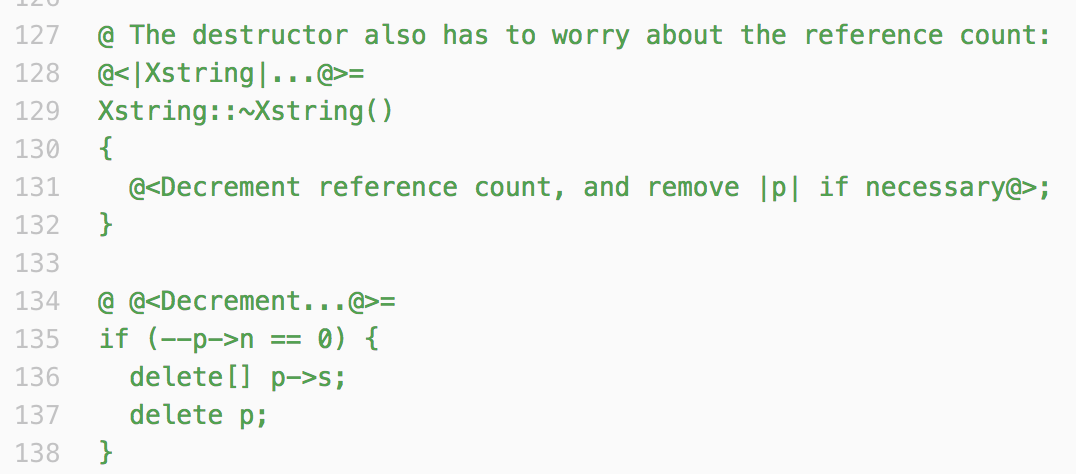
\includegraphics[width=8cm,height=5cm]{resources/fig_lp_file.png}%
	%\includegraphics[width=\textwidth]{conceptdriven.eps}
	\caption[Example of XString.w Literate Programming file in C++]{Example of XString.w Literate Programming file in C++ from [\cite{LPExample:XString}]} 
	\label{fig:XStringLPExample}
\end{figure}

LP provide advantages to software developers. This programming paradigm allows users to understand source code better. It provide a layer to help developers able to read both of natural language (NL) representation and programming language representation of the code. In example showed in Figure  \ref{fig:XStringLPExample}, developers know what action need to do for the destructor in the documentation part, which is decrementing value of a variable, and how to do the action by a decrement assignment and an if statement. Besides, LP helps developer read the documentation parts aligned with the programming parts, which they can check the explanation of behaviors of each program elements instead of reading the implementation and documentation separately. This way of representation make developers be able to imagine about how the source code work for each implementation parts and be able to debug the code easier. In overall, LP provides the more understandable form of source code, including what does the code do and how it works by descriptions in natural language  and descriptions in programming language .

\section{Challenges of realizing Literate Programming}
Realizing LP requires both representation of documentation and implementation parts for each source code file. There are two possible trends to derive these parts, however they faces the problems of effort consuming and low accuracy.
 
\subsection{Manually writing documentation and implementation}
Since the appearance in 1984, LP has not been applied as a popular programming language [\cite{LPArticle:MainStream1}] This fact is surprising since LP provides advantages for code understanding. According to ]cite{}, the main reason is that manually writing the code given documentation parts and manually documented the code given implementation parts are expensive tasks, especially with people who only have background in writing documentation or only have background in writing the code. 

For people who are focusing their work on writing software documentation, doing the implementation part of the documentation are usually infeasible task for them to complete. They know about what elements need to be defined or handled in the implementation and know how program elements involved implementation parts. However, their knowledge is represented by natural language. The most straight forward way for them is learning about programming language to have background of writing code. However, it is not a cheap stacks since it requires 4 years on average for training a Computer Science undergraduate student in the US. Natural Language and Programming Language has many differences how they abstracting the software explanation. For example, in natural language, people can use some indirect reference like pronoun such as "it", "they" while their is no such pronoun representation in some common programming languages like Java. Besides, people who are writing software requirements might need to work with projects in several languages instead of a single programming language, cause it is impossible for them to infer the implementation parts even if they already have background in one language.

From vice versa, people who have experiences in doing the implementation parts of the code might have more background to manually get the documents the code they write. This could be possible and recommended for any developers who are students to do the documents correspond to their small software projects, to make them understand the code better and check the bug in the code faster if bugs exist. However, in industrial projects which contains more than 1000 line of codes, the cost for writing documentation related to each parts of code are expensive, while it can slow down the development process of a software project as half, since developers need to write the explanation for the code they write. In addition, the code does not stay the same and code are updated days by days following requirements of users. This fact brought challenges for software developers to manually write documentation although they have good background for explaining the code in natural language. In overall, manually writing both documentation parts and implementation  are expensive. So that, approach for automatically deriving documentation and implementation are important.

\subsection{Automatically  inferring implementation by Machine Translation }
 In translation between natural languages, phrase based machine translation (PBMT) and Neural Machine Translation (NMT) are two common machine translation (MT) approaches that show their effectiveness for the inference problems. This fact brings MT as the most used translation engines [\cite{8416973}]. We might think about a solution for the software engineering is that applying MT to inferring implementation from documentation, given the intuition that both implementation and documentation have the same intension of describing how computer program works. However, researches on using MT in this area still not have good results yet [\cite{DBLP:journals/corr/BaroneS17}], due to several following problems.
\subsubsection{Lack of high quality Parallel corpus}
In natural language processing, current MT techniques rely on large scale corpus, which contains 10000 to millions pairs between different languages \cite{}. Machine learning algorithms like Bayesian learning are used to learn the mapping between source and target  languages. The corpus needed to be prepared as pairs of sentences, and the target languages need to be written manually by linguistic experts. However, in software engineering, building such a parallel corpus for documentation and implementation manually are expensive. 
Another approach is to relying on documentation written as natural language code comments. This seems to be a good direction since large scale code corpus contains millions line of code (LOC) and there are textual description in the form of code comments for each source code files. However, this type of documentation doesn't guarantee to have the same intent of describing the behavior of related source code. For example. this documentation contains "TODO" tags which are automatically generated by the IDE, or  contains comments that are actually source code which is commented by developers. In fact, such a corpus generated by documentation in the form of code comments and implementation contains noise and cause very low quality inference in MT models \cite{} .
Along with the problems from the shortage of good parallel corpus, MT also facing the problems from the differences between natural language and programming language, A survey \cite{} summarized the main differences between two languages which hindered an MT models for learning mapping between two languages. In general, it comes from the different purpose of translation between natural language processing and program generation, and more important, natural language and programming language have different mechanism of indirect reference management \cite{}.
\subsubsection{MT for Natural Language to Natural Language: Descriptive Model}
In Natural Language, the main purpose for inferring the target language is to helping user understand about the main idea of the source sentence. In the other words, it solved like providing the description for the content of source language, which include what is the main subject, what are the verbs and what are objects used in the sentence in a form of a sample subject-verb-object structure sentence. Let's see an example in figure \cite{}. In this example, which I observed from NMT system for Germany to English translation published by tensorflow \cite{}, the generated neural machine translation result shows almost the same with the expected sentence except one word "Halef" which is a last name. From this generated sentence, users can easily understand the meaning of the sentence and this kind of missing words error are acceptable. In NL, MT worked as a descriptive model, which allows thhe translated result missed one or two words compared to the expected sentence while users still understand.
\subsubsection{MT for Natural Language to Programming Language: Generative Model}
In contrast with NL-to-NL translation, the direction of natural language to programming language requires a very precise generated result. We can look at an example in figure \cite{}. SpecTrans \cite{} is a statistical machine translation system for inferring between documentation and implementation for java specification. The phase of inferring implementation returns 27 \% of syntactically correct. SpecTrans returns 38 \% of results are close to the expected result like this example. In the example in \cite{}, although we only used two edit actions to get the correct result, the translated implementation are still syntactically incorrect and cannot use directly as an generated source code. The problem of syntactically incorrect doesn't appear only in documentation to implementation translation but also in translating between object oriented programming languages. SemSMT \cite{} shows that there are over 60\% of translated results are syntactically incorrect. In overall, generating code from source, even if documentation or code from other programming language is an error-prone task by machine translation.
\subsubsection{Differences in indirect references between Natural Language and Programming Language}
\cite{} summarized problems of the generation of code from natural language of several existing tools. In general, the most important is that they have unique ways for handling indirect references. An example of such types of differences is shown by example \cite{}. In this example, a variable x can be described by the pronoun "it" in natural language as an indirect reference to variable x. However, in the implementation, there is only one way for represent variable x. These differences brings challenges for MT system to learn the mapping between languages. We will describe about types of indirect references between natural language and programming language in the next section.


\section{Direction of  a syntax-based approach for Natural Language to Programming Language translation}
Realizing Literate Programming can take benefits from a module for automatically generating code from documentation. However, the building of such a module based on machine translation engines used in natural language processing faced challenges. In this project, we analyze the problem from another aspect instead of relying on statistical approach. Our intuition is that, natural language description can be represented as a natural language parser by \cite{}, and each type of nodes in the parsed tree has rules for the translation by a syntax-based approach. To achieve this task, we conduct my research in the following steps.  First, according to survey \cite{}, we studied main problems of indirect references between two languages. Next, we studied each node types in Natural Language parser and propose rules for translation. After that, we implement a module that embedded these rules in an Natural Language Visitor based on the idea of ASTVisitor in programming language, to translate the code comment for each source files of a java project. We build a tool as an online IDE for users to do literate programming and publish on the site \cite{}. 










% Chapter 2 of the Thesis Template File
%   which includes bibliographic references.
\chapter{REVIEW OF LITERATURE}
In this chapter, we will overview main differences between NL versus PL and understand meaning of each natural language elements. To get this summarization of problems between two languages, we rely on problems between NL and PL listed in [\cite{Pulido-Prieto:2017:SNP:3145473.3109481}] and problems we found.
\section{Differences between Natural Language and Programming Language}
According to [\cite{Pulido-Prieto:2017:SNP:3145473.3109481}], programming language has limit language expressiveness while natural language description has stronger expressiveness.  In natural language, there are linguistic elements that have a different level of expressiveness compare to programming language.
\subsection{Deixis}
According to Oxford English Dictionary, "deixis" means "the function or use of deictic words or expressions whose meaning depends on where, when, or by whom they are used". In other words,this concept highlight that in natural language, there are words that their meaning depend on the context. Deixis are used to express the sentence in  shorter way without losing its meaning. In the direction of NL to PL, along with the context of NL, we have the context from the surrounding source code. \\

\begin{figure}[htp]
	\centering
	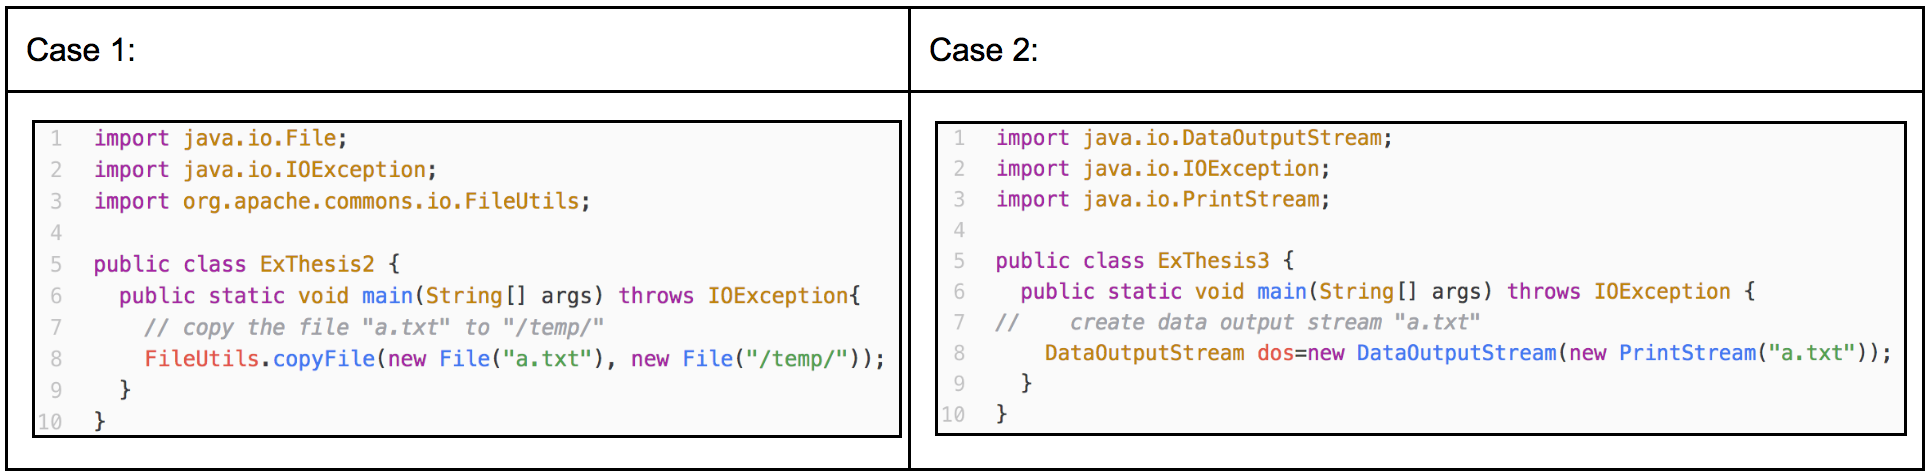
\includegraphics[width=17cm,height=6cm]{resources/fig_deixis_example.png}%
	%\includegraphics[width=\textwidth]{conceptdriven.eps}
	\caption[Example of Deixis in NL-to-PL translation]{Example of Deixis in NL-to-PL translation} 
	\label{fig:DeixisExample}
\end{figure}

An example of deixis is shown in the code snippet in Figure \ref{fig:DeixisExample}. In this example, "the file" here has the reference to the type "java.io.File". In this context, although the description mentioned only about a class name. There are several ways for describe an object by deixis, like using pronouns such as "it" or "they". In the other words, deixis provides a type of indirect reference between object in natural language and object in implementation. \\

Another example is case 2 in figure \ref{fig:DeixisExample}. In this example, the verb "create" will be understood as an constructor of the DataInputStream object, with the respected argument as a file name mentioned in the NL description. This case shows another example of indirect reference, which map a verb to a constructor statement in Java. There are multi types of deixis between NL and PL which hindered automatically approach like NMT to study this mapping based on the problem of indirect references. 

\subsection{Expressiveness}
In Oxford Dictionary, expressiveness means "showing or able to show your thoughts and feelings". In NL, expressiveness helps users to describe their ideas in many ways.  This is due to the fact that English can cover a large set of lexical rules, grammatical rules and textual rules. \cite{Pulido-Prieto:2017:SNP:3145473.3109481} shows that there are different set of rules between different subset language of English. In the area of NL to PL, natural languages have implicit references for expressing ideas while programming language used a very explicit references. For example, we can easily see natural language description contains "previous", "next" but in the corresponding implementation, we can only have number and variables. \\
\begin{figure}[htp]
	\centering
	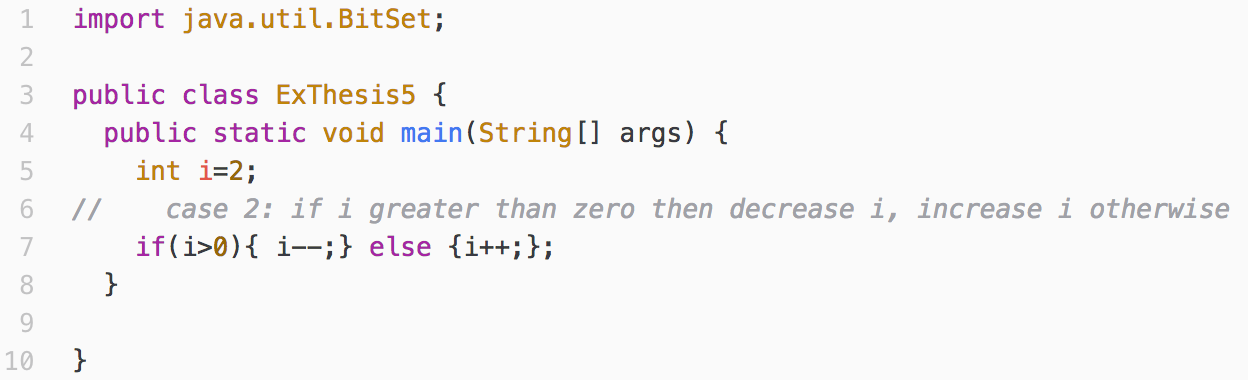
\includegraphics[width=14cm,height=5cm]{resources/fig_expressiveness_example.png}%
	%\includegraphics[width=\textwidth]{conceptdriven.eps}
	\caption[Example of Expressiveness in NL-to-PL translation]{Example of Expressiveness in NL-to-PL translation} 
	\label{fig:ExpressivenessExample}
\end{figure}
NL and PL have a very separate mechanism of managing the expressiveness in description related to control structures. An example of Expressiveness difference is shown in Figure \ref{fig_ExpressivenessExample}. In this example, the description mentioned about if and otherwise case about a boolean condition. However, in the implementation, the code for the implementation is the if-then-else structure. The order of description of statement of else branch is before the term "otherwise", while "else" keyword should be before this statement in the implementation. Along with basic control structure, we can face the problem of expressiveness in many other structure and algorithms, like loop and recursion. The different of expressiveness causes the mismatch between learning the control structure of programming language given the natural language description. 

\subsection{Phrases}
Natural Language description consists of one or more phrases. In NL to PL, each phrase may have a specific semantic  meaning related to variables and statements. Phrases can be very complex and can be ambiguous about their mapping in the PL. Several phrases can be mapped to one statement in the implementation, while several sentences can be mapped to single control structure. \\

\begin{figure}[htp]
	\centering
	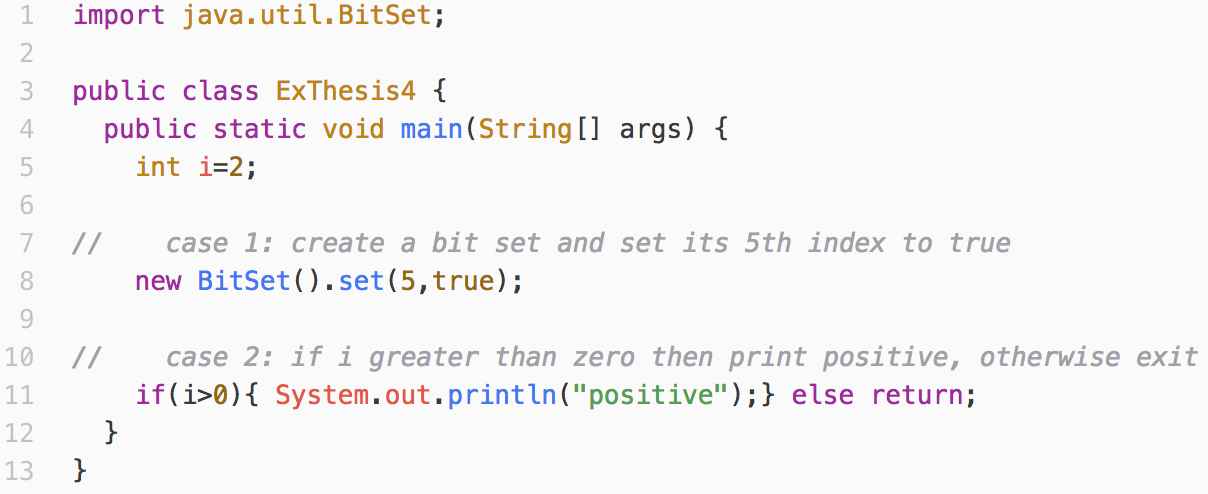
\includegraphics[width=14cm,height=6cm]{resources/fig_phrase_example.png}%
	%\includegraphics[width=\textwidth]{conceptdriven.eps}
	\caption[Example of Phrase Complexity in NL-to-PL translation]{Example of Phrase Complexity in NL-to-PL translation} 
	\label{fig:PhraseExample}
\end{figure}

In case 1 of example in Figure \ref{fig:PhraseExample}, we can see that two phrases of the description "create bit set and set its 5th index to true" corresponded to one method invocation, in which the first phrase is the receiver while the second phrase mentioned about the method identifier and expected method argument. The differences in phrase translation rules can be shown on the second case. In this example, two sentences in the documentation actually mentioned about an "If" branch and an "else" branch of an if statement. In general, the mapping of phrase to statement in NL to PL is not always be one to one mapping. The mapping rules between phrase in NL and statement in PL might depends on types of phrase along with context of NL description.
   
\subsection{Anaphoric Relations}
In natural languages, abstraction of types are not only in the form of class name like example we show in deixis but also in the form of providing description relate to class properties and methods. An example of anaphoric relations is  shown in example in Fiigure \ref{fig:AnaphoricExample}. In the NL description, a noun phrase "dog" actually refers to a class name and the verb "is barking" mentioned about method bark() defined inside a Dog class. This description implies about a validation for NL description, in which ensure that bark() has to be a method of Dog object. Depending on paradigm of programming language, the corresponding implementation may be differed. For example, in object-oriented language, we must assured that the project contains this description has definition of Dog class with bark() method, while in functional language like C or Pascal, we valid our program by finding a function bask() that accept a struct "Dog". \\

\begin{figure}[htp]
	\centering
	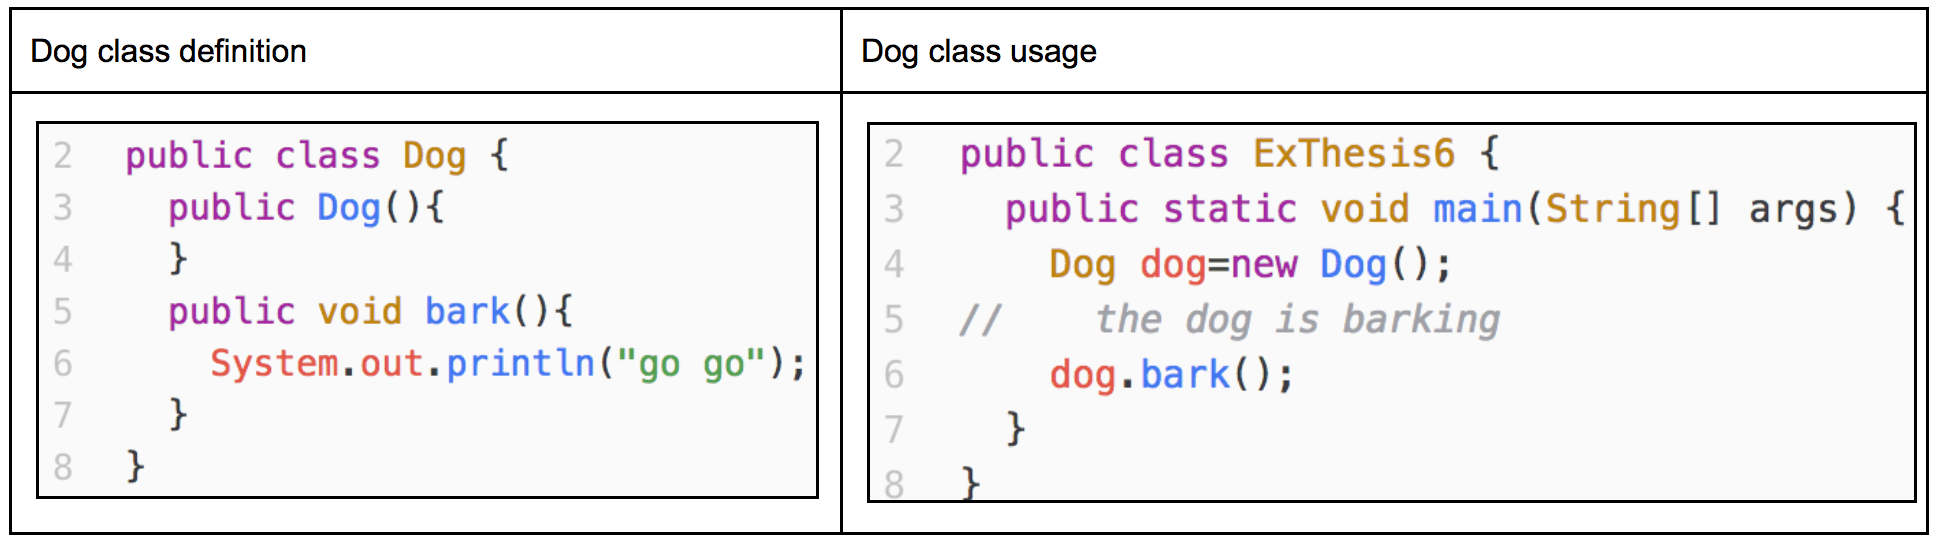
\includegraphics[width=18cm,height=6cm]{resources/fig_anaphoric_example.png}%
	%\includegraphics[width=\textwidth]{conceptdriven.eps}
	\caption[Example of Anaphoric Relation in NL-to-PL translation]{Example of Anaphoric Relation n NL-to-PL translation} 
	\label{fig:AnaphoricExample}
\end{figure}


Along with deixis, anaphoric relations provides the full support for indirect reference between NL and PL. While deixis relate to how to mention about a type information in form of class name only or pronoun, anaphoric relations focuses on expression every properties of an instance, including its methods and fields. A common of type of this relation is relation between verb to method invocation. When you see a verb in NL description along with a class name like Figure \ref{fig:AnaphoricExample}, it means that the corresponding implementation is about a method invocation of the class name in NL description.
 
\subsection{Context}
To realizing literate programming, context is an important element deciding the correctness of natural language to programming language translation. Unlike NL-to-NL translation which considered the context such as surrounding phrases or surrounding sentences given an input, the NL-to-PL considered both the natural language side and programming language side as context of given NL description. \\

Given a NL description, its related implementation might depend on surrounding NL description. In case 2 of example in Figure \ref{fig:PhraseExample}. the phrase "set its 5th index to true" has a translated result as a method invocation "set" of java.util.BitSet object. We know about the receiver of this implementation based on the previous phrase "create a bit set", which provides us information about a BitSet object. If we don't have the first phrase, we cannot inferred to the correct set method invocation, though we have method name along with parameters. \\

Along with context from NL part, information from programming language part brings an essential context for NL description. In case 2 of Figure  \ref{fig:PhraseExample}, we don't have information about the constructor of Bit Set. However, we can predict about the receiver of "set" method identifier based on the surrounding code, in which we have the information about a BitSet object. Context of PL parts provides all possible variables and class name are valid to use for the NL description. Context at PL level helps to restrict the implementation parts only relate to APIs that define in the scope of project, including its imported jar file and source code files. In our knowledge, current techniques for generating code from natural language considered the NL context as a full context and skip the information about surrounding code like AnyCode [\cite{Gvero:2015:SJE:2814270.2814295}] . In AnyCode, each NL description solved as a query for code instead of a comment, which hinders its ability for realizing literate programming, which requires NL descriptions consistent with surrounding NL context and PL context.

\subsection{Ambiguity}
Ambiguity in NL to PL translation means that one element in NL may has many interpretations, which the correct one may be varied based on the context. We can manually check to find the correct interpretation but an automatic translation engine doesn't have the ability to do that. To allow reasoning and de-ambiguous the translation result, we need to study types of ambiguity and design an algorithm for reasoning. In our knowledge, their are 2 important types of ambiguity in NL side and PL sides. \\

\begin{figure}[htp]
	\centering
	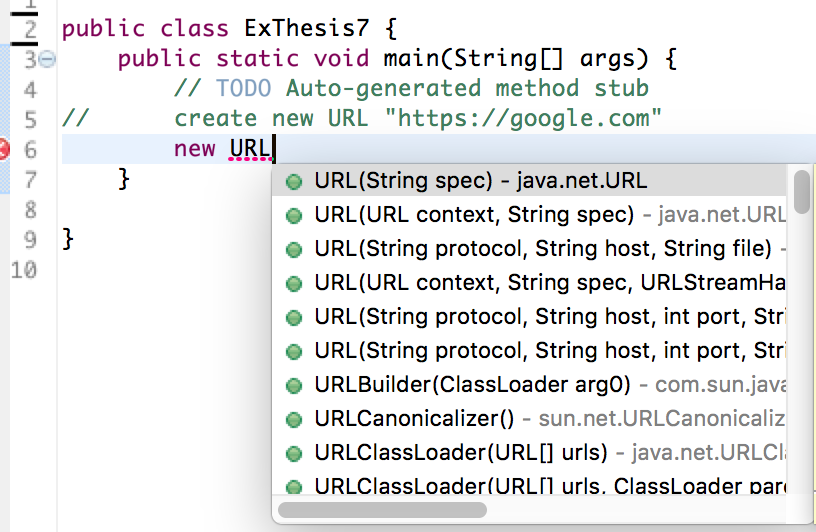
\includegraphics[width=14cm,height=6cm]{resources/fig_url_ambiguous_example.png}%
	%\includegraphics[width=\textwidth]{conceptdriven.eps}
	\caption[Example of URL type ambigous in NL-to-PL translation]{Example of URL type ambigous in NL-to-PL translation} 
	\label{fig:UrlAmbiguousExample}
\end{figure}

In NL side, noun and verb are two popular elements that have ambiguous in translated results. With noun, class name in NL might have more than one type annotation in PL. Information of correct type annotations can depend on the context of source file projects. In example show in Figure \ref{fig:UrlAmbiguousExample}, the class name "URL" has several type annotations, in which the most popular one is "java.net.URL", With verb, the ambiguity can happen between statement trigger or method invocation. In case 1 show on Figure \ref{fig:VerbAmbiguousExample}, the "set" verb is a assignment statement in the implementation, while in case 2 it is a method invocation set of Hash Map. There are several information from context can differentiate between two cases. In example one, the verb is used with a variable, a preposition "to" and a value that have the same type with a variable. In example two, the verb is used with two variable written consecutively. We can rely on such information to make correct reasoning.  \\

\begin{figure}[htp]
	\centering
	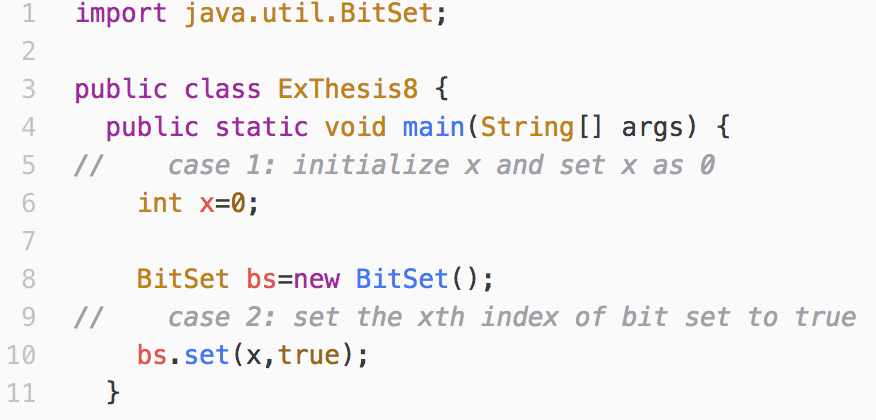
\includegraphics[width=14cm,height=6cm]{resources/fig_set_ambiguous_example.png}%
	%\includegraphics[width=\textwidth]{conceptdriven.eps}
	\caption[Example of verb ambigous in NL-to-PL translation]{Example of verb ambigous in NL-to-PL translation} 
	\label{fig:VerbAmbiguousExample}
\end{figure}

In PL side, ambiguous can happen between translating verb as method invocation. One verb can be translated to multiple invocations. In case 2 of example show in Figure \ref{}, there are in over 40 method APIs named "set" in libraries of JDK and apache common io. They have the same identifiers but their behavior are differed from each other, based on their receiver and argument. To reason the correct API for verbs, relying on the NL context including variables and value defined in the NL description might be a good direction. In overall, ambiguous is one of the most challenges for NL-to-PL translation, which make code query system like [\cite{Gvero:2015:SJE:2814270.2814295}] cannot be used for literate programming, since it doesn't use enough context in PL for reasoning the correct interpretation. 
     
\section{Elements  of a Natural Language parser}

Stanford-NLP [\cite{P13-1045}] is one of the most popular Natural Language Processing toolkits. The core of Stanford-NLP is based on its Stanford Parser. Stanford parser is a natural language parser, which analyses the grammatical structure of sentences and identifying type of words, such as verb, subject or object. Stanford Parser uses probabilistic parser, which uses information from corpus of sentences parsed manually to analyze new sentence. The output of this parser is an natural language parsed tree, which is important in NL to PL translation systems such as AnyCode [\cite{Gvero:2015:SJE:2814270.2814295}]. In this tree, each nodes will belong to one type of the Penn Treebank tags [\cite{Taylor2003}]. In this section, we study the purpose of each Treebank tags and its context in NL description for PL. In total, there are 82 tags defined in [\cite{Taylor2003}]. In these tags, 62 of them are frequently used in  NL description which are belong to 3 types: clause level, phrase level and word level. This section will introduce an overview of each NL tags.

\subsection{Clause level tags}
Clause level tags are elements for representing a grammar structure of sentences. The most frequent type of clause is the simple declarative clause which has abbreviation S. S is one of the basic clauses for conversation and writing [\cite{Cambridge:STag}]. The grammar of declarative sentence usually contains subject, verb and object. An example of S is shown in Figure \ref{fig:StagExample}. \\
\begin{figure}[htp]
	\centering
	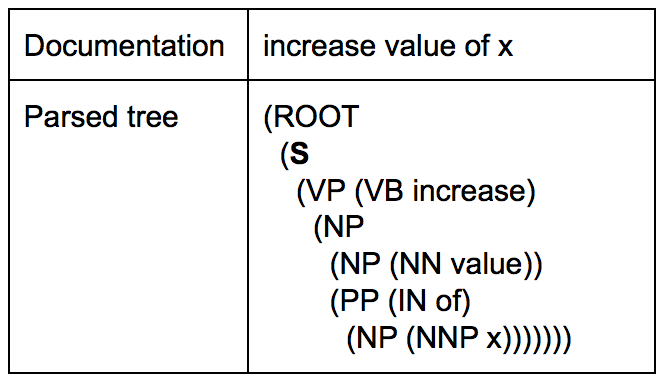
\includegraphics[width=8cm,height=4cm]{resources/fig_stag_example}
	\caption[Example of Simple declarative clause (S tag)] {Example of Simple declarative clause (S tag)}
	\label{fig:StagExample}
\end{figure}
Along with declarative sentence, NL grammar allows other types of sentences such as interrogate, imperative or exclamatory. There are 4 other types of clause defined by PennTree Bank: SBAR, SBARQ, SINV and SQ. SBAR stands for subordinate clause. It usually begin with subordinating conjunction along with a simple declarative clause. In NL description for PL, we can see SBAR frequently in the form of "if" clause. In case 1 example in Figure \ref{fig:SBARSBARQTagExample}, "if" solved as subordinating conjunction before description of boolean condition "x is greater than zero". SBARQ stands for direct question introduced by wh-word or wh-phrase. Since NL description is usually a description about behavior of implementation, SBARQ rarely see in NL to PL translation. SINV is the inverted declarative sentence, which usually has past tense verb in its content like case in example. SQ is a question that has yes/no answer options. Differ from SBARQ question, SQ sentences don't start with wh-element. Example of SBARQ tag is shown in case 2 of Figure \ref{fig:SBARSBARQTagExample}. 

\begin{figure}[htp]
	\centering
	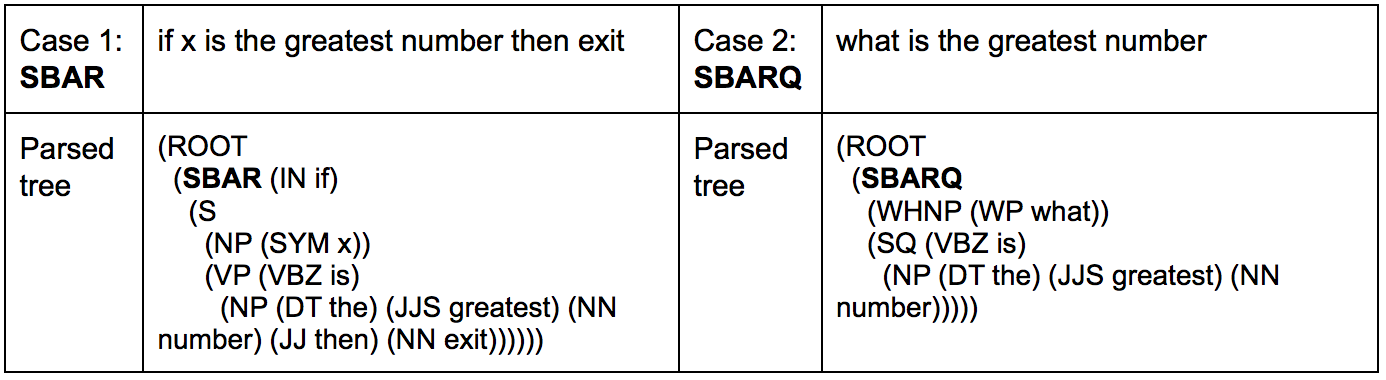
\includegraphics[width=14cm,height=4cm]{resources/fig_sbar_sbarq_2examples}
	\caption[Examples of SBAR and SBARQ tags] {Examples of SBAR and SBARQ tags}
	\label{fig:SBARSBARQTagExample}
\end{figure}

\subsection{Phrase level tags}
Phrase level tags are usually at non-terminal level of NL tree. Each types of phrase level tags consist element at leaf node as word level. In table \ref{table:SummarizeAllTags}, we show the list of phrase level tags along with examples.
\begin{longtable}{|p{.05\textwidth}|p{.15\textwidth}|p{.10\textwidth}|p{.35\textwidth}|p{.35\textwidth}|}
% Please add the following required packages to your document preamble:
% \usepackage[table,xcdraw]{xcolor}
% If you use beamer only pass "xcolor=table" option, i.e. \documentclass[xcolor=table]{beamer}
 \caption[]{Semantic explanation of Penn-Tree Bank tags and  their popularity in NL description (red block as popular, green block as normally and yellow block as rarely used)}
\label{table:SummarizeAllTags} \\
		\hline
		\rowcolor[HTML]{38FFF8} 
		\multicolumn{1}{|c|}{\cellcolor[HTML]{38FFF8}\textbf{No}} & \multicolumn{1}{c|}{\cellcolor[HTML]{38FFF8}\textbf{Level}} & \multicolumn{1}{c|}{\cellcolor[HTML]{38FFF8}\textbf{Tags}} & \multicolumn{1}{c|}{\cellcolor[HTML]{38FFF8}\textbf{Meaning in NL description}}                                 & \multicolumn{1}{c|}{\cellcolor[HTML]{38FFF8}\textbf{Example as NL description}} \\ \hline
		\rowcolor[HTML]{FFCCC9} 
		1                                                         & Clause level                                                & S                                                          & - simple declarative clause- Usually use for mention about statements                                           & increase value of x                                                             \\ \hline
		\rowcolor[HTML]{FFCCC9} 
		2                                                         & Clause level                                                & SBAR                                                       & - Clause introduced by a (possibly empty) subordinating conjunction.- Usually relate to if statement            & if x is the greatest number then exit                                           \\ \hline
		\rowcolor[HTML]{9AFF99} 
		3                                                         & Clause level                                                & SBARQ                                                      & - Direct question introduced by a wh-word or a wh-phrase.- Usually use for mentions about statements            & what is the greater number                                                      \\ \hline
		\rowcolor[HTML]{9AFF99} 
		4                                                         & Clause level                                                & SINV                                                       & - Inverted declarative sentence- Usually use for mentions about statements                                      & given to x was a value that was equal to length to array                        \\ \hline
		\rowcolor[HTML]{9AFF99} 
		5                                                         & Clause level                                                & SQ                                                         & - Inverted yes/no question- Usually relate to check condition                                                   & does x greater than zero?                                                       \\ \hline
		\rowcolor[HTML]{FFCCC9} 
		6                                                         & Phrase level                                                & ADJP                                                       & Adjective Phrase.                                                                                               & the value of x is negative.                                                     \\ \hline
		\rowcolor[HTML]{FFCCC9} 
		7                                                         & Phrase level                                                & ADVP                                                       & - Adverb Phrase.- Adverb Phrases Show How, Where, Why, When                                                     & why do we increase the value of x?                                              \\ \hline
		\rowcolor[HTML]{FFCCC9} 
		8                                                         & Phrase level                                                & CONJP                                                      & Conjunction Phrase.                                                                                             & dog and cat and fox are animals.                                                \\ \hline
		\rowcolor[HTML]{FFFFC7} 
		9                                                         & Phrase level                                                & FRAG                                                       & - Fragment (sentence that miss subjects and/or verbs).- Usually use in dialog, not so popular in NL description & From morning until night.                                                       \\ \hline
		\rowcolor[HTML]{FFFFC7} 
		10                                                        & Phrase level                                                & INTJ                                                       & - Interjection (for strong emotion) - Not popular in NL description                                             & Hello! How are you?                                                             \\ \hline
		\rowcolor[HTML]{FFFFC7} 
		11                                                        & Phrase level                                                & LST                                                        & - List marker. Includes surrounding punctuation.- Not popular in NL description                                 & 1) 2)                                                                           \\ \hline
		\rowcolor[HTML]{FFFFC7} 
		12                                                        & Phrase level                                                & NAC                                                        & - Not a Constituent- Not popular in NL description                                                              &                                                                                 \\ \hline
		\rowcolor[HTML]{FFCCC9} 
		13                                                        & Phrase level                                                & NP                                                         & - Noun Phrase.- Usually use for describe class name or variables                                                & the array is created                                                            \\ \hline
		\rowcolor[HTML]{9AFF99} 
		14                                                        & Phrase level                                                & NX                                                         & - Used within certain complex NPs to mark the head of the NP. - Not popular in NL description                   &                                                                                 \\ \hline
		\rowcolor[HTML]{9AFF99} 
		15                                                        & Phrase level                                                & PP                                                         & - Prepositional Phrase.- Usually connect words between APIs or variables                                        & read value from console                                                         \\ \hline
		\rowcolor[HTML]{9AFF99} 
		16                                                        & Phrase level                                                & PRN                                                        & - Parenthetical.                                                                                                & x (the integer value) is initialized                                            \\ \hline
		\rowcolor[HTML]{9AFF99} 
		17                                                        & Phrase level                                                & PRT                                                        & - Particle- Use with little or no meaning                                                                       & move the chess up one position                                                  \\ \hline
		\rowcolor[HTML]{9AFF99} 
		18                                                        & Phrase level                                                & QP                                                         & - Quantifier Phrase; used within NP.- Might use for describe loop                                               & every ten minutes, this method runs in a thread.                                \\ \hline
		\rowcolor[HTML]{FFFFC7} 
		19                                                        & Phrase level                                                & RRC                                                        & - Reduced Relative Clause.- Not popular in NL description                                                       & the variable we created will be used in the future.                             \\ \hline
		\rowcolor[HTML]{FFFFC7} 
		20                                                        & Phrase level                                                & UCP                                                        & - Unlike Coordinated Phrase.- Not popular in NL description.                                                    &                                                                                 \\ \hline
		\rowcolor[HTML]{FFCCC9} 
		21                                                        & Phrase level                                                & VP                                                         & - Verb Phrase.- Usually use for represent statements, operations and method invocations.                        & increase value of x                                                             \\ \hline
		\rowcolor[HTML]{9AFF99} 
		22                                                        & Phrase level                                                & WHADJP                                                     & Wh-adjective Phrase                                                                                             & how does it work                                                                \\ \hline
		\rowcolor[HTML]{9AFF99} 
		23                                                        & Phrase level                                                & WHAVP                                                      & Wh-adverb Phrase.                                                                                               & why do I increase x                                                             \\ \hline
		\rowcolor[HTML]{9AFF99} 
		24                                                        & Phrase level                                                & WHNP                                                       & Wh-noun Phrase.                                                                                                 & we calculate how many candies in a box.                                         \\ \hline
		\rowcolor[HTML]{9AFF99} 
		25                                                        & Phrase level                                                & WHPP                                                       & Wh-prepositional Phrase. Prepositional phrase containing a wh-noun phrase.                                      & we create a console then we get the value of x from which.                      \\ \hline
		\rowcolor[HTML]{FFFFC7} 
		26                                                        & Phrase level                                                & X                                                          & - Unknown, uncertain, or unbracketable.- Not popular in NL description.                                         &                                                                                 \\ \hline
		\rowcolor[HTML]{FFCCC9} 
		27                                                        & Word level                                                  & CC                                                         & coordinating conjunction                                                                                        & and                                                                             \\ \hline
		\rowcolor[HTML]{9AFF99} 
		28                                                        & Word level                                                  & CD                                                         & cardinal number                                                                                                 & 1, third                                                                        \\ \hline
		\rowcolor[HTML]{9AFF99} 
		29                                                        & Word level                                                  & DT                                                         & determiner                                                                                                      & the                                                                             \\ \hline
		\rowcolor[HTML]{9AFF99} 
		30                                                        & Word level                                                  & EX                                                         & existential there                                                                                               & there is                                                                        \\ \hline
		\rowcolor[HTML]{9AFF99} 
		31                                                        & Word level                                                  & FW                                                         & foreign word                                                                                                    & les                                                                             \\ \hline
		\rowcolor[HTML]{9AFF99} 
		32                                                        & Word level                                                  & IN                                                         & preposition, subordinating conjunction                                                                          & in, of, like                                                                    \\ \hline
		\rowcolor[HTML]{9AFF99} 
		33                                                        & Word level                                                  & IN/that                                                    & that as subordinator                                                                                            & that                                                                            \\ \hline
		\rowcolor[HTML]{9AFF99} 
		34                                                        & Word level                                                  & JJ                                                         & adjective                                                                                                       & green                                                                           \\ \hline
		\rowcolor[HTML]{9AFF99} 
		35                                                        & Word level                                                  & JJR                                                        & adjective, comparative                                                                                          & greener                                                                         \\ \hline
		\rowcolor[HTML]{9AFF99} 
		36                                                        & Word level                                                  & JJS                                                        & adjective, superlative                                                                                          & greenest                                                                        \\ \hline
		\rowcolor[HTML]{9AFF99} 
		37                                                        & Word level                                                  & LS                                                         & list marker                                                                                                     & 1)                                                                              \\ \hline
		\rowcolor[HTML]{9AFF99} 
		38                                                        & Word level                                                  & MD                                                         & modal                                                                                                           & could, will                                                                     \\ \hline
		\rowcolor[HTML]{FFCCC9} 
		39                                                        & Word level                                                  & NN                                                         & noun, singular or mass                                                                                          & table                                                                           \\ \hline
		\rowcolor[HTML]{FFCCC9} 
		40                                                        & Word level                                                  & NNS                                                        & noun plural                                                                                                     & tables                                                                          \\ \hline
		\rowcolor[HTML]{FFCCC9} 
		41                                                        & Word level                                                  & NNP                                                        & proper noun, singular                                                                                           & David                                                                           \\ \hline
		\rowcolor[HTML]{FFCCC9} 
		42                                                        & Word level                                                  & NNPS                                                       & proper noun, plural                                                                                             & Iowans                                                                          \\ \hline
		\rowcolor[HTML]{FFFFC7} 
		43                                                        & Word level                                                  & PDT                                                        & predeterminer                                                                                                   & both the variables                                                              \\ \hline
		\rowcolor[HTML]{FFFFC7} 
		44                                                        & Word level                                                  & POS                                                        & possessive ending                                                                                               & friend’s                                                                        \\ \hline
		\rowcolor[HTML]{9AFF99} 
		45                                                        & Word level                                                  & PP                                                         & personal pronoun                                                                                                & I, he, it                                                                       \\ \hline
		\rowcolor[HTML]{FFFFC7} 
		46                                                        & Word level                                                  & PP\$                                                       & possessive pronoun                                                                                              & my, his                                                                         \\ \hline
		\rowcolor[HTML]{9AFF99} 
		47                                                        & Word level                                                  & RB                                                         & adverb                                                                                                          & however, usually, naturally, here, good                                         \\ \hline
		\rowcolor[HTML]{9AFF99} 
		48                                                        & Word level                                                  & RBR                                                        & adverb, comparative                                                                                             & better                                                                          \\ \hline
		\rowcolor[HTML]{9AFF99} 
		49                                                        & Word level                                                  & RBS                                                        & adverb, superlative                                                                                             & best                                                                            \\ \hline
		\rowcolor[HTML]{9AFF99} 
		50                                                        & Word level                                                  & RP                                                         & particle                                                                                                        & give up                                                                         \\ \hline
		\rowcolor[HTML]{9AFF99} 
		51                                                        & Word level                                                  & SENT                                                       & Sentence-break punctuation                                                                                      & . ! ?                                                                           \\ \hline
		\rowcolor[HTML]{9AFF99} 
		52                                                        & Word level                                                  & SYM                                                        & Symbol                                                                                                          & / {[} = *                                                                       \\ \hline
		\rowcolor[HTML]{9AFF99} 
		53                                                        & Word level                                                  & TO                                                         & infinitive ‘to’                                                                                                 & togo                                                                            \\ \hline
		\rowcolor[HTML]{FFCCC9} 
		54                                                        & Word level                                                  & VB                                                         & verb be, base form                                                                                              & be                                                                              \\ \hline
		\rowcolor[HTML]{FFCCC9} 
		55                                                        & Word level                                                  & VBD                                                        & verb be, past tense                                                                                             & was, were                                                                       \\ \hline
		\rowcolor[HTML]{FFCCC9} 
		56                                                        & Word level                                                  & VBG                                                        & verb be, gerund/present participle                                                                              & being                                                                           \\ \hline
		\rowcolor[HTML]{FFCCC9} 
		57                                                        & Word level                                                  & VBN                                                        & verb be, past participle                                                                                        & been                                                                            \\ \hline
		\rowcolor[HTML]{FFCCC9} 
		58                                                        & Word level                                                  & VBP                                                        & verb be, sing. present, non-3d                                                                                  & am, are                                                                         \\ \hline
		\rowcolor[HTML]{FFCCC9} 
		59                                                        & Word level                                                  & VBZ                                                        & verb be, 3rd person sing. present                                                                               & is                                                                              \\ \hline
		\rowcolor[HTML]{9AFF99} 
		60                                                        & Word level                                                  & VH                                                         & verb have, base form                                                                                            & have                                                                            \\ \hline
		\rowcolor[HTML]{9AFF99} 
		61                                                        & Word level                                                  & VHD                                                        & verb have, past tense                                                                                           & had                                                                             \\ \hline
		\rowcolor[HTML]{9AFF99} 
		62                                                        & Word level                                                  & VHG                                                        & verb have, gerund/present participle                                                                            & having                                                                          \\ \hline
		\rowcolor[HTML]{9AFF99} 
		63                                                        & Word level                                                  & VHN                                                        & verb have, past participle                                                                                      & had                                                                             \\ \hline
		\rowcolor[HTML]{9AFF99} 
		64                                                        & Word level                                                  & VHP                                                        & verb have, sing. present, non-3d                                                                                & have                                                                            \\ \hline
		\rowcolor[HTML]{9AFF99} 
		65                                                        & Word level                                                  & VHZ                                                        & verb have, 3rd person sing. present                                                                             & has                                                                             \\ \hline
		\rowcolor[HTML]{9AFF99} 
		66                                                        & Word level                                                  & VV                                                         & verb, base form                                                                                                 & take                                                                            \\ \hline
		\rowcolor[HTML]{9AFF99} 
		67                                                        & Word level                                                  & VVD                                                        & verb, past tense                                                                                                & took                                                                            \\ \hline
		\rowcolor[HTML]{9AFF99} 
		68                                                        & Word level                                                  & VVG                                                        & verb, gerund/present participle                                                                                 & taking                                                                          \\ \hline
		\rowcolor[HTML]{9AFF99} 
		69                                                        & Word level                                                  & VVN                                                        & verb, past participle                                                                                           & taken                                                                           \\ \hline
		\rowcolor[HTML]{9AFF99} 
		70                                                        & Word level                                                  & VVP                                                        & verb, sing. present, non-3d                                                                                     & take                                                                            \\ \hline
		\rowcolor[HTML]{9AFF99} 
		71                                                        & Word level                                                  & VVZ                                                        & verb, 3rd person sing. present                                                                                  & takes                                                                           \\ \hline
		\rowcolor[HTML]{9AFF99} 
		72                                                        & Word level                                                  & WDT                                                        & wh-determiner                                                                                                   & which                                                                           \\ \hline
		\rowcolor[HTML]{9AFF99} 
		73                                                        & Word level                                                  & WP                                                         & wh-pronoun                                                                                                      & who, what                                                                       \\ \hline
		\rowcolor[HTML]{9AFF99} 
		74                                                        & Word level                                                  & WP\$                                                       & possessive wh-pronoun                                                                                           & whose                                                                           \\ \hline
		\rowcolor[HTML]{9AFF99} 
		75                                                        & Word level                                                  & WRB                                                        & wh-abverb                                                                                                       & where, when                                                                     \\ \hline
        
       
\end{longtable}

\subsection{Word level tags}
Clause level tags are node at terminal level in NL tree. The list of each word level tags and example are shown in table \ref{table:SummarizeAllTags}. 
In NL to PL translation, noun, verb preposition and conjunction are the most important tags used for NL description. Noun group usually represents for class name and variables, with plural or non-plural. Verb are used as statement trigger or method invocation description.Preposition is usually used as the connector between variables in the context of arguments in a method invocation, while conjunction responds to the connection between phrase in NL. Group of adjective and adverb are usually used for representing properties of a class or an object instance.


% Chapter 3 from the thesis template file
%   that contains an example table and figure.
\chapter{METHODS AND PROCEDURES}
In the previous chapter, we discuss main problems of NL to PL translation and elements of NL Parser, which are different types of tags for building an NL parse tree representation for NL sentence. These knowledge help us for gaining background to design our syntax-based approach for NL to PL translation. while NLP researches relies on analyzing NL parsed tree, we also considered NL parsed tree for NL description as the core element for translation. To handle the syntax of NL parsed tree, we relied on how programming language handled an Abstract Syntax Tree (AST) which is a representation of a source code file by building ASTVisitor. Based on ideas of ASTVisitor in PL, we designed the NLPLVisitor for NL to PL translation.  
\section{Designing a NLPL Visitor}
\subsection{Visitor Pattern}
In programming language design, collections are most important data types. A collection may have instances from multiple types. Since we usually use loop for handling information from collection, it is very common that we need to write an operation or method to handle each element of collection without knowing the type of each elements. There is one way to write an operation, which used "instanceof" condition to check the type of each elements in a collection, however this way is not reflecting object oriented design. 

A pattern that allows handle element of different types inside a collection in object oriented way calls Visitor pattern. In a visitor pattern, developers have the ability for representing operations on each types of elements of a collection. Besides, it allows you to write new operation without interfering the previous operations you define for types of element. In other words, visitor pattern overcomes the conflict between object structure s and algorithm  which the the object structure operates on, means you can update the algorithm handling for each elements without changing the structure of element. Along with collections, visitor pattern is also available for other data type structures such as tree structure.

One of the most useful data structure for handling source code is Abstract-Syntax- Tree (AST). In AST tree, each node in tree belong to a specific node type depend on the source code. An example of AST is shown on figure \cite{}. In this example, "println" is a method invocation node which contains elements as its child node like a String literal argument. Obviously, to handle content of AST, we need to have an visitor pattern for taking operation on each type of nodes. ASTVisitor, which is developed by eclipse JDT (\cite{})is an important implementation of visitor pattern for operating the AST tree.

A design diagram of ASTVisitor is shown as follows. ASTVisitor is the name of the interface in package of eclipse JDT. It has several operation defined for each type of AST node, the most important operation is the visit() method declaration. There are set of method visit() in ASTVisitor, which each method take a specific type of ASTNode as type of its argument and each method will execute some algorithms based on type of ASTNode. To handle the operation on ASTNode on our own, we need to define a class that implements ASTVisitor and define content inside body of each visit operation. Our own visitor can be passed as an argument of ASTParser, which is used to produce the ASTNode for the whole source code and storing information of our visitor. A full class diagram of an ASTVisitor is shown on figure \cite{}.
 
\subsection{NLPLVisitor}
Inspiring from advantages of ASTVisitor in programming language, we use a visitor pattern for design a module for dealing with the complexity of Natural Language parsed tree in NL to PL translation. NL parsed tree, to be remind, is a data structure for representing NL description in the form of a tree in which each node belongs to a specific tags in a tag sets of Penn Tree bank we discussed in the previous chapter. Similar to handling AST tree in PL, we design and implement an abstract class NLPL Visitor which we defined the basic visit method declaration for all types of NL tags. Then, we defined implementation of each visit operation relates to each type by writing a class that implements the NLPL visitor. Since our work is for translating between two languages, we called this implemented class Translation Visitor. 

Considering the translation can be done by a syntax based approach, we implement the content of each visit function as follows. First, we need to understand the intuition of each NL tags in the translation to PL. Next, we provide rules for each NL tags for translating to get  elements in PL. In this step, we considered the children of each NL node and its terminal (textual value) as the most important information to decide which rules will be used for the translation of the node. The intuition of each NL tags is provided based on our observations on the NL description corpus as documentation of Java Development Kit (JDK), and the summarization of them are shown in figure \cite{}. The implemented rules for each NL tags will be discussed in the next section.

\section{Solving Problems between Natural Language and Programming Language}
\subsection{Context: Extracting Information from Variable and Literal}
Context of NL description is information that can be mentioned in it. We consider surrounding code of NL description in a source code file and al Java APIs that can be accessible by a Java project that contains the description are two resources for representing the context of source code. In NLPL, given input of java project, NLPL has a module for extracting all accessible APIs in this project. They are APIs from imported library and APIs defined in each source files. The algorithm for extracting all accessible APIs is shown in figure \cite{}. \\
In NL side,an NL description usually mentions about information of variable and literal value along with class name. We consider ambiguous types of class name is one type of indirect reference and we handle that by a reasoning module in the next section. For variables, we get information of all accessible variables in a set of variable object extract by algorithm \cite{} and check in NL description if it mentioned about a variable or not. For literal, we check if NL description contains a literal value by regular expression. We define regular expressions for string value and numeric value to do the checking. \\
One problems of NL parser is that it relied on probabilistic parsing, so it can be error-prone. By looking at examples of NL descriptions and see the results of NL parser manually, we identify that keeping variable and literal in original form caused parsing with not useful information. For example, in the code showed in figure \cite{}, we see that a string value "text.txt" broke into 3 parts in NL parser, while we should consider it as a single element for processing. Similarly, with example 2 on figure \cite{}, the variable "a" is parsed to be a node of verb, which is not correct. To overcome this problem which cause by non-useful tags and incorrect tags, we represented variables and literal as an unique alias by the last step of preprocessing step in algorithm \cite{}. An example of unique alias is shown in the example of algorithm.  

\subsection{NL Tree Transformation}
The appearance of variable and literal inside NL description leads to our observation is that, in NL descriptions, some part can be considered as textual node while other parts are actually expressions like variable and literal. The expression parts can be used directly when composing to the final results for translation. This fact motivates us to transform the original parsed tree to a transformed tree with 2 types of nodes: Textual node and Expression node. This transformation allows us to embedding information specifically depends on node. An example of NL Tree transformation is shown on figure \cite{}.  In this example, we are able to embed information about variable a such as its type, its scope  as local variable inside an Expression node. The class diagram of Textual Node and Expression is shown on figure \cite{}. Both Expression node and Textual node will have information about NL tags, they keep all informations from original NL parsed tree. Since the final output for NLPL is source code which can be expressions or statement, the transformed tree served as a representation of a bridge language which connect information between source language and target language. The idea of bridge language has been applied in Natural Language translations such as for English, French or Russian \cite{}.

\subsection{Phrase: Connecting information between each Phrase in translation}
We handle complexity in phrase level by the idea that we need to find a way to combine translation results of each phrases in NL description. We consider conjunction tags CC, such as "and" or "or" are two main elements that separate between each phrase in translation.  In NL description, we consider that both "and" and "or" are usually used between boolean literal for expressing logical operator. In addition, "and" is usually used for combining translated results of each single phrase. We handle the "and" and the "or" conjunctions by algorithm shown in figure \cite{}. \\
An example of different usage of "and" conjunction is shown by 3 examples in figure \cite{}. In the first example, we have "and" appears between two  boolean expressions that are used for comparison. In this case, due to the translated result is boolean for each single phrase, then the final translated result of "and" will be "\&\&" operator. In the second example, we see that the translated result for the first single clause is a constructor and the type of the constructor is the type of receiver of method API in the second clause. In this case, the combineExpression() function will mix translated results of these two phrases into a single expression. The thrid example shows a different condition compared to example 2. In this case, the constructor in the first clause doesn't have the same type with neither receiver and arguments. In this case the combineExpression() function will return 2 expressions consecutively as the final translated result.  \\
In the first 3 sections, we propose algorithms for take advantages of context in NL to PL translation and reasoning on on complex phrases, which are two per six main problems of naturalistic programming (\cite{}). In next sections, we will introduce our solution for solving four remaining problems which relate to Indirect reference: deixis, expressiveness, anaphoric relation and ambiguity.
\subsection{Rules for translating Natural Language elements}
In the NLPLVisitor, we provide rules for handling each NL tags. The main idea is that we identify types of tags, what children tags it produce then provide rules and its terminal value. An overview of rules and function relate to each tags is shown in table \cite{}.
\subsection{Solving IR on Noun Phrase as class name}

\subsubsection{Identifying  class name as Noun Phrase}
\subsubsection{Resolving types for  class name}
\subsection{Solving IR on Verb Phrase as Statement Trigger}
\subsection{Solving IR on Verb Phrase as Method Invocation}
\subsection{Solving IR on Preposition as Method API}

\subsection{NLPL Architecture Overview}



% Chapter 4 from the standard thesis template
%   that contains an adv. example table and figure.
 \addtocontents{toc}{\protect\newpage}
\chapter{EXPERIMENTAL}
In this section, I want to answer on the research question: How well NLPL performs for translating from Natural Language comments to code.  
\section{Data Preparation}

\section{Experiment Result}

\begin{table}[]
	\begin{tabular}{|l|l|l|l|l|}
		\hline
		\textbf{K} & \textbf{AnyCode} & \textbf{NLPL} & \textbf{Top-K of AnyCode} & \textbf{Top-K of NLPL} \\ \hline
		1              & 32               & 39            & 61.54\%                   & 75.00\%                \\ \hline
		2              & 39               & 40            & 75.00\%                   & 76.92\%                \\ \hline
		3              & 41               & 41            & 78.85\%                   & 78.85\%                \\ \hline
		4              & 42               & 42            & 80.77\%                   & 80.77\%                \\ \hline
		5              & 45               & 42            & 86.54\%                   & 80.77\%                \\ \hline
	\end{tabular}
\end{table}

\begin{longtable}{|p{.10\textwidth}|p{.35\textwidth}|p{.40\textwidth}|p{.15\textwidth}|}
% Please add the following required packages to your document preamble:
% \usepackage[table,xcdraw]{xcolor}
% If you use beamer only pass "xcolor=table" option, i.e. \documentclass[xcolor=table]{beamer}
		\hline
		\multicolumn{1}{|c|}{\textbf{No}} & \multicolumn{1}{c|}{\textbf{Natural Language Comment}} & \multicolumn{1}{c|}{\cellcolor[HTML]{FFCCC9}\textbf{NLPL Top-1 result}}                                          & \multicolumn{1}{c|}{\textbf{Top-K Acc}} \\ \hline
		&                                                        & \multicolumn{1}{c|}{\cellcolor[HTML]{9AFF99}\textbf{Expected result}}                                            &                                         \\ \hline
		\rowcolor[HTML]{FFCCC9} 
		1                                 & copy file fname to destination                         & FileUtils .copyFile( new File( fname ) ,new File( destination ) )                                                & 1                                       \\ \hline
		\rowcolor[HTML]{9AFF99} 
		&                                                        & FileUtils .copyFile(new File(fname), new File(destination))                                                      &                                         \\ \hline
		\rowcolor[HTML]{FFCCC9} 
		2                                 & load class "MyClass.class"                             & Thread .currentThread() .getContextClassLoader() .loadClass( "MyClass .class" )                                  & 1                                       \\ \hline
		\rowcolor[HTML]{9AFF99} 
		&                                                        & Thread .currentThread() .getContextClassLoader() .loadClass(”MyClass .class”)                                    &                                         \\ \hline
		\rowcolor[HTML]{FFCCC9} 
		3                                 & make file ”text.txt”                                   & new LineNumberReader(new InputStreamReader( new File( "text .txt" ) )) .ready()                                  & 4                                       \\ \hline
		\rowcolor[HTML]{9AFF99} 
		&                                                        & new File(”text .txt”) .createNewFile()                                                                           &                                         \\ \hline
		\rowcolor[HTML]{FFCCC9} 
		4                                 & write "hello" to file "text.txt"                       & FileUtils .writeStringToFile( new File( "text .txt" ) , "hello" )                                                & 1                                       \\ \hline
		\rowcolor[HTML]{9AFF99} 
		&                                                        & FileUtils .writeStringToFile(new File(”text .txt”), ”hello”)                                                     &                                         \\ \hline
		\rowcolor[HTML]{FFCCC9} 
		5                                 & new buffered reader ”text.txt”                         & new BufferedReader(new InputStreamReader( "text .txt" ))                                                         & 1                                       \\ \hline
		\rowcolor[HTML]{9AFF99} 
		&                                                        & new BufferedReader(new InputStreamReader("text .txt"))                                                           &                                         \\ \hline
		\rowcolor[HTML]{FFCCC9} 
		6                                 & open connection ”http://www.oracle.com/”               & new URL( "http://www .oracle .com/" ) .openConnection()                                                          & 1                                       \\ \hline
		\rowcolor[HTML]{9AFF99} 
		&                                                        & new URL(”http://www .oracle .com/”) .openConnection()                                                            &                                         \\ \hline
		\rowcolor[HTML]{FFCCC9} 
		7                                 & create socket ”http://www.oracle.com/” 80              & new Socket( "http://www .oracle .com/" , 80 )                                                                    & 1                                       \\ \hline
		\rowcolor[HTML]{9AFF99} 
		&                                                        & new Socket(”http://www .oracle .com/”, 80)                                                                       &                                         \\ \hline
		\rowcolor[HTML]{FFCCC9} 
		8                                 & put a pair ”Mike” , ”+41-345-89-23” into a map         & new HashMap() .put( "Mike" , "+41-345-89-23" )                                                                   & 1                                       \\ \hline
		\rowcolor[HTML]{9AFF99} 
		&                                                        & new HashMap() .put(”Mike”, ”+41-345-89-23”)                                                                      &                                         \\ \hline
		\rowcolor[HTML]{FFCCC9} 
		9                                 & set thread max priority                                & Thread .currentThread() .setPriority(Thread .MAX\_PRIORITY )                                                     & 1                                       \\ \hline
		\rowcolor[HTML]{9AFF99} 
		&                                                        & Thread .currentThread() .setPriority(Thread .MAX\_PRIORITY);                                                     &                                         \\ \hline
		\rowcolor[HTML]{FFCCC9} 
		10                                & set property ”gate.home” to value ”http://gate.ac.uk/” & new Properties() .setProperty( "gate .home" , "http://gate .ac .uk/" )                                           & 1                                       \\ \hline
		\rowcolor[HTML]{9AFF99} 
		&                                                        & new Properties() .setProperty(”gate .home”, ”http://gate .ac .uk/”)                                              &                                         \\ \hline
		\rowcolor[HTML]{FFCCC9} 
		11                                & does the file 'text.txt' exist                         & new File( "text .txt" )  .exists()                                                                               & 1                                       \\ \hline
		\rowcolor[HTML]{9AFF99} 
		&                                                        & new File("text .txt") .exists( )                                                                                 &                                         \\ \hline
		\rowcolor[HTML]{FFCCC9} 
		12                                & get thread id                                          & Thread .currentThread() .getId()                                                                                 & 1                                       \\ \hline
		\rowcolor[HTML]{9AFF99} 
		&                                                        & Thread .getCurrentThread() .getId()                                                                              &                                         \\ \hline
		\rowcolor[HTML]{FFCCC9} 
		13                                & join thread                                            & Thread .currentThread() .join()                                                                                  & 1                                       \\ \hline
		\rowcolor[HTML]{9AFF99} 
		&                                                        & Thread .getCurrentThread() .join()                                                                               &                                         \\ \hline
		\rowcolor[HTML]{FFCCC9} 
		14                                & delete file ”text.txt”                                 & FileDeleteStrategy .NORMAL .delete(new File( "text .txt" ) )                                                     & 1                                       \\ \hline
		\rowcolor[HTML]{9AFF99} 
		&                                                        & new File(”text .txt”) .delete()                                                                                  &                                         \\ \hline
		\rowcolor[HTML]{FFCCC9} 
		15                                & print exception ex stack trace                         & ex  .printStackTrace()                                                                                           & 1                                       \\ \hline
		\rowcolor[HTML]{9AFF99} 
		&                                                        & ex .printStackTrace()                                                                                            &                                         \\ \hline
		\rowcolor[HTML]{FFCCC9} 
		16                                & is ”text.txt” directory                                & new File( "text .txt" ) .isDirectory()                                                                           & 1                                       \\ \hline
		\rowcolor[HTML]{9AFF99} 
		&                                                        & new File(”text .txt”) .isDirectory()                                                                             &                                         \\ \hline
		\rowcolor[HTML]{FFCCC9} 
		17                                & get thread stack trace                                 & Thread .currentThread() .getStackTrace()                                                                         & 1                                       \\ \hline
		\rowcolor[HTML]{9AFF99} 
		&                                                        & Thread .currentThread() .getStackTrace()                                                                         &                                         \\ \hline
		\rowcolor[HTML]{FFCCC9} 
		18                                & read line by line file ”text.txt”                      & new LineNumberReader(new InputStreamReader( new File( "text .txt" ) )) .readLine()                               & 1                                       \\ \hline
		\rowcolor[HTML]{9AFF99} 
		&                                                        & FileUtils .readLines(new File(”text .txt”))                                                                      &                                         \\ \hline
		\rowcolor[HTML]{FFCCC9} 
		19                                & set time zone to ”GMT”                                 & Calendar .getInstance() .setTimeZone(TimeZone .getTimeZone( "GMT" ) )                                            & 1                                       \\ \hline
		\rowcolor[HTML]{9AFF99} 
		&                                                        & Calendar .getInstance() .setTimeZone(TimeZone .getTimeZone(”GMT”))                                               &                                         \\ \hline
		\rowcolor[HTML]{FFCCC9} 
		20                                & free memory                                            & Runtime .getRuntime() .freeMemory()                                                                              & 1                                       \\ \hline
		\rowcolor[HTML]{9AFF99} 
		&                                                        & Runtime .getRuntime() .freeMemory()                                                                              &                                         \\ \hline
		\rowcolor[HTML]{FFCCC9} 
		21                                & total memory                                           & Runtime .getRuntime() .totalMemory()                                                                             & 1                                       \\ \hline
		\rowcolor[HTML]{9AFF99} 
		&                                                        & Runtime .getRuntime() .totalMemory()                                                                             &                                         \\ \hline
		\rowcolor[HTML]{FFCCC9} 
		22                                & new data input stream ”text.txt”                       & new DataInputStream(new FileInputStream( "text .txt" ))                                                          & 1                                       \\ \hline
		\rowcolor[HTML]{9AFF99} 
		&                                                        & new DataInputStream(new FileInputStream(”text .txt”))                                                            &                                         \\ \hline
		\rowcolor[HTML]{FFCCC9} 
		23                                & rename file ”text1.txt” to ”text2.txt”                 & new File( "text1 .txt" )  .renameTo(new File( "text2 .txt" ) )                                                   & 1                                       \\ \hline
		\rowcolor[HTML]{9AFF99} 
		&                                                        & new File(”text1 .txt”) .renameTo(new File(”text2 .txt”))                                                         &                                         \\ \hline
		\rowcolor[HTML]{FFCCC9} 
		24                                & move file ”text1.txt” to ”text2.txt”                   & FileUtils .moveFile( new File( "text1 .txt" ) ,new File( "text2 .txt" ) )                                        & 1                                       \\ \hline
		\rowcolor[HTML]{9AFF99} 
		&                                                        & FileUtils .moveFile(new File(”text1 .txt”), new File(”text2 .txt”))                                              &                                         \\ \hline
		\rowcolor[HTML]{FFCCC9} 
		25                                & read utf from the file ”text.txt”                      & FileUtils .readFileToString(new File( "text .txt" ) )                                                            & 2                                       \\ \hline
		\rowcolor[HTML]{9AFF99} 
		&                                                        & new DataInputStream(new FileInputStream(”text .txt”)) .readUTF()                                                 &                                         \\ \hline
		\rowcolor[HTML]{FFCCC9} 
		26                                & set thread min priority                                & Thread .currentThread() .setPriority(Thread .MIN\_PRIORITY )                                                     & 1                                       \\ \hline
		\rowcolor[HTML]{9AFF99} 
		&                                                        & Thread .currentThread() .setPriority(Thread .MIN PRIORITY)                                                       &                                         \\ \hline
		\rowcolor[HTML]{FFCCC9} 
		27                                & create panel and set layout to border                  & new Panel()  .setLayout(new BorderLayout() )                                                                     & 1                                       \\ \hline
		\rowcolor[HTML]{9AFF99} 
		&                                                        & new Panel() .setLayout(new BorderLayout())                                                                       &                                         \\ \hline
		\rowcolor[HTML]{FFCCC9} 
		28                                & sort array                                             & Arrays .sort( array )                                                                                            & 1                                       \\ \hline
		\rowcolor[HTML]{9AFF99} 
		&                                                        & Arrays .sort(array)                                                                                              &                                         \\ \hline
		\rowcolor[HTML]{FFCCC9} 
		29                                & add label ”Names:” to panel                            & new Panel() .add( new Label( "Names:" ) )                                                                        & 1                                       \\ \hline
		\rowcolor[HTML]{9AFF99} 
		&                                                        & new Panel() .add(new Label(”Names:”))                                                                            &                                         \\ \hline
		\rowcolor[HTML]{FFCCC9} 
		30                                & write 2015 to data output stream ”text.txt”            & new DataOutputStream(new FileOutputStream( "text .txt" ))  .writeInt( 2015 )                                     & 1                                       \\ \hline
		\rowcolor[HTML]{9AFF99} 
		&                                                        & new DataOutputStream(new FileOutputStream(”text .txt”)) .write(2015)                                             &                                         \\ \hline
		\rowcolor[HTML]{FFCCC9} 
		31                                & get date when file ”text.txt” was last time modified   & new File( "text .txt" )  .lastModified()                                                                         & \textgreater{}10                        \\ \hline
		\rowcolor[HTML]{9AFF99} 
		&                                                        & new Date(new File(”text .txt”) .lastModified()) .getTime()                                                       &                                         \\ \hline
		\rowcolor[HTML]{FFCCC9} 
		32                                & check file ”text.txt” ”read” permission                & AccessController .checkPermission(new FilePermission( "text .txt" , "read" ) )                                   & 1                                       \\ \hline
		\rowcolor[HTML]{9AFF99} 
		&                                                        & AccessController .checkPermission(new FilePermission(”text .txt”, ”read”))                                       &                                         \\ \hline
		\rowcolor[HTML]{FFCCC9} 
		33                                & read lines with numbers from file ”text.txt”           & new LineNumberReader(new InputStreamReader( new File( "text .txt" ) )) .readLine()                               & 1                                       \\ \hline
		\rowcolor[HTML]{9AFF99} 
		&                                                        & new LineNumberReader(new InputStreamReader(new FileInputStream(”text .txt”))) .readLine()                        &                                         \\ \hline
		\rowcolor[HTML]{FFCCC9} 
		34                                & read from console                                      & new BufferedReader(new InputStreamReader( System .in )) .read()                                                  & 1                                       \\ \hline
		\rowcolor[HTML]{9AFF99} 
		&                                                        & new BufferedReader(new InputStreamReader(System .in)) .readLine()                                                &                                         \\ \hline
		\rowcolor[HTML]{FFCCC9} 
		35                                & is file ”text.txt” data available                      & new DataInputStream(new FileInputStream( new File( "text .txt" ) )) .available()                                 & 1                                       \\ \hline
		\rowcolor[HTML]{9AFF99} 
		&                                                        & new DataInputStream(new FileInputStream(”text .txt”)) .available()                                               &                                         \\ \hline
		\rowcolor[HTML]{FFCCC9} 
		36                                & get double value x                                     & Integer .valueOf( x ) .doubleValue()                                                                             & \textgreater{}10                        \\ \hline
		\rowcolor[HTML]{9AFF99} 
		&                                                        & Double .valueOf(x) .doubleValue()                                                                                &                                         \\ \hline
		\rowcolor[HTML]{FFCCC9} 
		37                                & write object o to file output stream ”data.obj"        & new ObjectOutputStream(new BufferedOutputStream(new FileOutputStream( "data .obj" ))) .writeObject( o )          & 1                                       \\ \hline
		\rowcolor[HTML]{9AFF99} 
		&                                                        & new ObjectOutputStream(new BufferedOutputStream(new FileOutputStream(”data .obj”))) .writeObject(o)              &                                         \\ \hline
		\rowcolor[HTML]{FFCCC9} 
		38                                & create bit set and set its 5th element to true         & new BitSet()  .set( 5 , true )                                                                                   & 1                                       \\ \hline
		\rowcolor[HTML]{9AFF99} 
		&                                                        & new BitSet() .set(5,true)                                                                                        &                                         \\ \hline
		\rowcolor[HTML]{FFCCC9} 
		39                                & accept request on port 80                              & new ServerSocket( 80 ) .accept()                                                                                 & 1                                       \\ \hline
		\rowcolor[HTML]{9AFF99} 
		&                                                        & new ServerSocket(80) .accept()                                                                                   &                                         \\ \hline
		\rowcolor[HTML]{FFCCC9} 
		40                                & get thread group                                       & Thread .currentThread() .getThreadGroup()                                                                        & 1                                       \\ \hline
		\rowcolor[HTML]{9AFF99} 
		&                                                        & Thread .currentThread() .getThreadGroup()                                                                        &                                         \\ \hline
		\rowcolor[HTML]{FFCCC9} 
		41                                & create panel and set layout to grid                    & new Panel()  .setLayout(new GridLayout() )                                                                       & \textgreater{}10                        \\ \hline
		\rowcolor[HTML]{9AFF99} 
		&                                                        & new Panel() .setLayout(new GridBagLayout())                                                                      &                                         \\ \hline
		\rowcolor[HTML]{FFCCC9} 
		42                                & get screen size                                        & Toolkit .getDefaultToolkit() .getScreenSize()                                                                    & 1                                       \\ \hline
		\rowcolor[HTML]{9AFF99} 
		&                                                        & Toolkit .getDefaultToolkit() .getScreenSize()                                                                    &                                         \\ \hline
		\rowcolor[HTML]{FFCCC9} 
		43                                & get splash screen graphics                             & ? .getSplashScreen()                                                                                             & \textgreater{}10                        \\ \hline
		\rowcolor[HTML]{9AFF99} 
		&                                                        & SplashScreen .getSplashScreen() .createGraphics()                                                                &                                         \\ \hline
		\rowcolor[HTML]{FFCCC9} 
		44                                & get display refresh rate                               & GraphicsEnvironment .getLocalGraphicsEnvironment() .getDefaultScreenDevice() .getDisplayMode() .getRefreshRate() & 1                                       \\ \hline
		\rowcolor[HTML]{9AFF99} 
		&                                                        & GraphicsEnvironment .getLocalGraphicsEnvironment() .getDefaultScreenDevice() .getDisplayMode() .getRefreshRate() &                                         \\ \hline
		\rowcolor[HTML]{FFCCC9} 
		45                                & get keystroke modifiers                                & keystroke  .getModifiers()                                                                                       & 1                                       \\ \hline
		\rowcolor[HTML]{9AFF99} 
		&                                                        & KeyEvent .getKeyModifiersText(keystroke .getModifiers())                                                         &                                         \\ \hline
		\rowcolor[HTML]{FFCCC9} 
		46                                & generate ”RSA” private key                             & new Thread( "RSA" ) .yield()                                                                                     & \textgreater{}10                        \\ \hline
		\rowcolor[HTML]{9AFF99} 
		&                                                        & KeyPairGenerator .getInstance(”RSA”) .generateKeyPair() .getPrivate()                                            &                                         \\ \hline
		\rowcolor[HTML]{FFCCC9} 
		47                                & reverse list                                           & Collections .reverseOrder()                                                                                      & \textgreater{}10                        \\ \hline
		\rowcolor[HTML]{9AFF99} 
		&                                                        & Collections .reverse(list)                                                                                       &                                         \\ \hline
		\rowcolor[HTML]{FFCCC9} 
		48                                & intersection of rectangle 4 5 with rectangle 3 2       & ? .intersection(? )                                                                                              & \textgreater{}10                        \\ \hline
		\rowcolor[HTML]{9AFF99} 
		&                                                        & new Rectangle(5, 4) .intersection(new Rectangle(3, 2))                                                           &                                         \\ \hline
		\rowcolor[HTML]{FFCCC9} 
		49                                & set cursor over label to hand                          & new AffineTransform() .setToIdentity()                                                                           & \textgreater{}10                        \\ \hline
		\rowcolor[HTML]{9AFF99} 
		&                                                        & label .setCursor(Cursor .getPredefinedCursor(Cursor .HAND CURSOR))                                               &                                         \\ \hline
		\rowcolor[HTML]{FFCCC9} 
		50                                & read big integer from console                          & new BufferedReader(new InputStreamReader( System .in )) .read()                                                  & 3                                       \\ \hline
		\rowcolor[HTML]{9AFF99} 
		&                                                        & new Scanner(System .in) .nextBigInteger()                                                                        &                                         \\ \hline
		\rowcolor[HTML]{FFCCC9} 
		51                                & delete file ”text.txt” when JVM terminates             & new File( "text .txt" )  .delete()                                                                               & \textgreater{}10                        \\ \hline
		\rowcolor[HTML]{9AFF99} 
		&                                                        & new File(”text .txt”) .deleteOnExit()                                                                            &                                         \\ \hline
		\rowcolor[HTML]{FFCCC9} 
		52                                & get date instance for Germany                          & DateFormat .getDateTimeInstance() .getDateInstance()                                                             & \textgreater{}10                        \\ \hline
		\rowcolor[HTML]{9AFF99} 
		&                                                        & DateFormat .getDateTimeInstance(DateFormat .MEDIUM,DateFormat .MEDIUM, Locale .GERMANY)                          &                                         \\ \hline
		
\end{longtable}

\section{Result Analysis}

\section{NLPL Online IDE}




% Chapter 5 from the standard thesis template
%   with a full page figure and a sideways table.
\chapter{SUMMARY AND DISCUSSION}



%% Rearranging the table of contents to show references before appendix
%\unappendixtitle
%\addcontentsline{toc}{chapter}{REFERENCES} %this line is to be included before the last chapter so that in toc it appears after the last chapter. If you want the reference to be the last entry of the toc, remove this line and in the biblio.tex file insert this line (or uncomment the line  )
% An example bibliography from the standard thesis template
\renewcommand{\bibname}{\centerline{REFERENCES}}
\unappendixtitle
\interlinepenalty=300
% For no page break use thebibnopage environment
\bibliography{Reference/references}
\bibliographystyle{ieeetr}
% Appendix1 file from standard thesis template
\appendixtitle
\appendix
\chapter{ADDITIONAL MATERIAL}

This is now the same as any other chapter except that
all sectioning levels below the chapter level must begin
with the *-form of a sectioning command.

\section*{More stuff}

Supplemental material.


% An example second appendix from the example thesis thesis.tex.
\chapter{STATISTICAL RESULTS}

This is now the same as any other chapter except that
all sectioning levels below the chapter level must begin
with the *-form of a sectioning command.

\section*{Supplemental Statistics}

More stuff.

%\renewcommand{\bibname}{\centerline{BIBLIOGRAPHY}}
\unappendixtitle
\newpage
\phantomsection
\addcontentsline{toc}{chapter}{BIBLIOGRAPHY}



\end{document}

% IMPORTANT NOTES
% TABLE OF CONTENTS :
% TOPIC 1:  If you need a page break follow the steps below
% step1
% check before which chapter in the table of contents you want a page break
% step 2
% go the folder "body". There open the chapter tex file that you noted needed page break in the table of contents..
% step 3
% insert  \addtocontents{toc}{\protect\newpage} before the first line i.e. before the line \chapter{RESULTS}.

% TOPIC 2: Rearrage the reference before or after the appendix where the include statements are given and it 
% gets rearranged in the toc
% 
% subtopic:  Including the references before the appendix only in the table of contents and not actually
% Step 1: Go to the last chapter of your thesis
% Step 2: Copy paste the following lines
%
% % Rearranging the table of contents to show references before appendix
% \unappendixtitle
% \addcontentsline{toc}{chapter}{REFERENCES} %this line is to be included before the last chapter so that in toc it appears after  the last chapter. If you want the reference to be the last entry of the toc, remove this line and in the biblio.tex file insert this line (or uncomment the line  )
%%%%%%%%%%%%%%%%%%%%%%%%%%%%
% \def\@makechapterhead#1{%   
% IN ORDER TO MAKE spacing changes in the title page got to the section in the isuthesis.cls file
% that starts with \long\def\maketitle{\begin{titlepage} and you can use options like
% singlespace (less spacing)
%singlespacing (comparitively more spacing almost like 2 spacing)
% onehalfspacing
%doublespacing (this is more spacing than the singlespacing above )
% more definitions on spacing can be found by going through the class file

